\documentclass[man]{apa6}
\usepackage{lmodern}
\usepackage{amssymb,amsmath}
\usepackage{ifxetex,ifluatex}
\usepackage{fixltx2e} % provides \textsubscript
\ifnum 0\ifxetex 1\fi\ifluatex 1\fi=0 % if pdftex
  \usepackage[T1]{fontenc}
  \usepackage[utf8]{inputenc}
\else % if luatex or xelatex
  \ifxetex
    \usepackage{mathspec}
  \else
    \usepackage{fontspec}
  \fi
  \defaultfontfeatures{Ligatures=TeX,Scale=MatchLowercase}
\fi
% use upquote if available, for straight quotes in verbatim environments
\IfFileExists{upquote.sty}{\usepackage{upquote}}{}
% use microtype if available
\IfFileExists{microtype.sty}{%
\usepackage{microtype}
\UseMicrotypeSet[protrusion]{basicmath} % disable protrusion for tt fonts
}{}
\usepackage{hyperref}
\hypersetup{unicode=true,
            pdftitle={Infants prefer to listen to speech: A meta-analysis.},
            pdfauthor={Cécile Issard, Sho Tsuji, \& Alejandrina Cristia},
            pdfkeywords={Meta-analysis, infants, speech preference, auditory development, natural
sounds},
            pdfborder={0 0 0},
            breaklinks=true}
\urlstyle{same}  % don't use monospace font for urls
\usepackage{graphicx,grffile}
\makeatletter
\def\maxwidth{\ifdim\Gin@nat@width>\linewidth\linewidth\else\Gin@nat@width\fi}
\def\maxheight{\ifdim\Gin@nat@height>\textheight\textheight\else\Gin@nat@height\fi}
\makeatother
% Scale images if necessary, so that they will not overflow the page
% margins by default, and it is still possible to overwrite the defaults
% using explicit options in \includegraphics[width, height, ...]{}
\setkeys{Gin}{width=\maxwidth,height=\maxheight,keepaspectratio}
\IfFileExists{parskip.sty}{%
\usepackage{parskip}
}{% else
\setlength{\parindent}{0pt}
\setlength{\parskip}{6pt plus 2pt minus 1pt}
}
\setlength{\emergencystretch}{3em}  % prevent overfull lines
\providecommand{\tightlist}{%
  \setlength{\itemsep}{0pt}\setlength{\parskip}{0pt}}
\setcounter{secnumdepth}{0}
% Redefines (sub)paragraphs to behave more like sections
\ifx\paragraph\undefined\else
\let\oldparagraph\paragraph
\renewcommand{\paragraph}[1]{\oldparagraph{#1}\mbox{}}
\fi
\ifx\subparagraph\undefined\else
\let\oldsubparagraph\subparagraph
\renewcommand{\subparagraph}[1]{\oldsubparagraph{#1}\mbox{}}
\fi

%%% Use protect on footnotes to avoid problems with footnotes in titles
\let\rmarkdownfootnote\footnote%
\def\footnote{\protect\rmarkdownfootnote}


  \title{Infants prefer to listen to speech: A meta-analysis.}
    \author{Cécile Issard\textsuperscript{1}, Sho Tsuji\textsuperscript{2}, \&
Alejandrina Cristia\textsuperscript{1}}
    \date{}
  
\shorttitle{Preference for speech sounds in infancy}
\affiliation{
\vspace{0.5cm}
\textsuperscript{1} Laboratoire de Sciences Cognitives et Psycholinguistique, Ecole Normale Supérieure, Département d'Études Cognitives\\\textsuperscript{2} International Research Center for Neurointelligence, The University of Tokyo}
\keywords{Meta-analysis, infants, speech preference, auditory development, natural sounds\newline\indent Word count: X}
\usepackage{csquotes}
\usepackage{upgreek}
\captionsetup{font=singlespacing,justification=justified}

\usepackage{longtable}
\usepackage{lscape}
\usepackage{multirow}
\usepackage{tabularx}
\usepackage[flushleft]{threeparttable}
\usepackage{threeparttablex}

\newenvironment{lltable}{\begin{landscape}\begin{center}\begin{ThreePartTable}}{\end{ThreePartTable}\end{center}\end{landscape}}

\makeatletter
\newcommand\LastLTentrywidth{1em}
\newlength\longtablewidth
\setlength{\longtablewidth}{1in}
\newcommand{\getlongtablewidth}{\begingroup \ifcsname LT@\roman{LT@tables}\endcsname \global\longtablewidth=0pt \renewcommand{\LT@entry}[2]{\global\advance\longtablewidth by ##2\relax\gdef\LastLTentrywidth{##2}}\@nameuse{LT@\roman{LT@tables}} \fi \endgroup}


\DeclareDelayedFloatFlavor{ThreePartTable}{table}
\DeclareDelayedFloatFlavor{lltable}{table}
\DeclareDelayedFloatFlavor*{longtable}{table}
\makeatletter
\renewcommand{\efloat@iwrite}[1]{\immediate\expandafter\protected@write\csname efloat@post#1\endcsname{}}
\makeatother
\usepackage{lineno}

\linenumbers

\authornote{

Correspondence concerning this article should be addressed to Cécile
Issard, Laboratoire de Sciences Cognitives et Psycholinguistique,
Département d'Études Cognitives, Ecole Normale Supérieure, 29 rue d'Ulm,
75005 Paris, France. E-mail:
\href{mailto:cecile.issard@gmail.com}{\nolinkurl{cecile.issard@gmail.com}}}

\abstract{
The human auditory system is amazingly efficient at processing speech.
Some works suggest that this capacity is present from birth, infants
preferring to listen to natural speech than to other types of sounds,
enabling them to select the signals that are relevant for communication
with conspecifics. However, in experimental studies, a large variety of
sounds have been contrasted to speech, with infants of very different
ages. Drawing a global picture of how this capacity emerges is therefore
difficult. We synthesized the literature by conducting a meta-analysis
of studies testing speech preference in infants from birth to one year
of age. We found a medium effect size, with infants preferring speech
over any other type of sound. Contrary to the results of individual
studies, we found no effect of age: infants showed the same amount of
preference from birth to one year of age. Still contrary to what
individual studies suggested, we found the same amount of preference
whether speech was contrasted to other natural sounds or to artificial
sounds; as well as whether speech was contrasted to other vocal sounds
or to non-vocal sounds. Preference was stronger when the speech stimuli
were in the infants' native language. This suggests that the
representation of speech as a distinct auditory object comes fromis
modulated by the degree of familiarity with the sounds of the language
they are exposed to.


}

\begin{document}
\maketitle

\section{Introduction}\label{introduction}

Speech is the main signal for human vocal communication. Adult
individuals efficiently detect speech sounds in their environment, and
use them to spot conspecifics and build social interactions. Since
seminal experimental results suggest that infants react more to speech
than to certain other sounds (Ecklund-Flores \& Turkewitz, 1996), it is
conceivable that newborns are equipped with a preference for speech
sounds, and that human infants become further entrenched in this
preference as they age and gain additional exposure to speech. Here, we
synthesize empirical data on infants' preferences for speech over
artificial sounds, natural sounds, as well as human non-speech sounds,
with the hope of illuminating the strength of evidence supporting
various theories proposed to explain infants' preferential listening and
processing studies. {[}insert Figure 1 here{]}

\subsection{Potential dimensions underlying preference
patterns}\label{potential-dimensions-underlying-preference-patterns}

There are three key conceptual explanations for infants preference for
speech: (a) Preference for natural over artificial sounds; (b)
preference for vocal over non-vocal sounds; and (c) preference for
familiar over unfamiliar sounds (see Figure 1 for a representation of
these distinctions). These three explanations are mutually compatible,
such that one or more may be found to be true. In this section, we
explain how these explanations differ, and briefly review some results
on each, before turning to the potential effects of age.

\subsubsection{Natural versus artificial
sounds}\label{natural-versus-artificial-sounds}

Natural sounds are those produced with biological systems, including
vocal tracts but also the sound of walking and heart rate. Inspection of
their acoustic characteristics reveals that in many cases natural and
artificial sounds may not have the same structure. For example, backward
speech has unnatural formant transitions and seemingly abrupt closures
that are not found in naturally produced sounds. We know that natural
sounds are processed more accurately by the auditory system, from the
cochlea (Lewicki, 2006) to the auditory cortex (e.g.~Gehr et al., 2000;
see Mizrahi et al., 2014 for a review). As a result, we can expect a
preference for speech over artificial sounds that is present from birth
and stable over age, predictions that seem to be validated in a first
glance of the literature (Vouloumanos \& Werker, 2007; Vouloumanos,
2014).

\subsubsection{Familiarity}\label{familiarity}

An alternative to the above explanation could be proposed based on
familiarity: Perhaps infants prefer speech to foils when these vary in
the level of familiarity, since artificial sounds may be less common
(and thus less familiar to the infants) than natural sounds. There are
no behavioral results directly testing the prediction that infants show
stronger preferences when tested with more familiar speech stimuli (for
instance, spoken in their native, as compared to a foreign language),
but results from neuroimaging studies do predict indirect evidence for
this view. For instance, newborns' brain activation was different for
forward than to backward speech when the native language was used as the
speech stimuli, but not when a foreign language was used (Sato et al.,
2012; May et al., 2018).

\subsubsection{Vocal versus non-vocal
sounds}\label{vocal-versus-non-vocal-sounds}

Many results summarized above may be accommodated by a third hypothesis,
postulating a preference for vocal over non-vocal sounds. Vocal sounds
are those made with a mouth, and thus typically a subset of natural
sounds. There is some evidence which is easy to explain with this
hypothesis but cannot be predicted from the natural sound preference or
the familiarity preference: Newborns made more head-turns to speech than
to heartbeat (Ecklund-Flores \& Turkewitz, 1996), but they listened
equivalently to speech and monkey calls (Vouloumanos \& Werker, 2010).
Arguably, speech and heartbeat are equally natural and they are both
familiar to a newborn and thus this result cannot be accommodated by
either of the other explanations. Changes as a function of development

When infants are born at term, they have already experienced speech and
natural sounds more generally for about three months (and throughout
their auditory lifelong experience). While little is known about
production experience in utero and how this may affect their perception
of sounds as being vocal, it is certain that newborns will have
experienced their native speech, which other work suggests newborns
prefer to prosodically distinct foreign speech (REF). The latter finding
actually suggests a potential inconsistency in findings in this body of
literature: While the preference for native over foreign speech is
consistent with the familiarity preference discussed above, this
familiarity may also predict a preference for native speech over monkey
vocalizations, which has not obtained (REF). In fact, 1- to 4-month-old
infants responded more to speech than to other human sounds (Shultz \&
Vouloumanos, 2010). To complicate matters further, one study reports
that 9-month-olds listened longer to monkey calls than speech
(Sorcinelli et al., 2019), which is in stark contradiction with a
preference systematically driven by familiarity. Setting this issue
aside, it remains clear that as infants age, they gain experience with
stimuli in their environment as well as their own vocal production. In
addition to the effects of experience, development of the auditory
pathway may affect perception (e.g., Mazuka, XX, \& Tsuji, 2018). These
age-related changes may affect the preference for speech in various
ways. One of them is by infants' developing an increasingly narrow and
precise definition of the spoken stimulus they prefer. Indeed, whereas
newborns do not prefer speech over monkey calls, three-month-olds do
(Vouloumanos et al., 2010). If the definition of speech becomes
increasingly narrow, it is conceivable that some of the naturalness,
familiarity, and vocal quality effects would change as a function of
age, such that very close stimuli (e.g., speech versus another natural
sound) initially leads to a weak preference, but, as infants age, this
preference may be as strong as that found for very different stimuli
(e.g., speech versus an artificial sound). While many articles discuss
potential changes in the pattern of preference as a function of age
(e.g.~Ferry et al., 2013; Shultz \& Vouloumanos, 2010; Shultz et al.,
2014), only two papers from the same laboratory that we know of includes
multiple age groups tested with the exact same stimuli and procedure
(Vouloumanos et al., 2010; Vouloumanos \& Werker, 2004), such that
comparisons are often done using the demonstrably problematic method of
stating \enquote{there is a difference here but not there, therefore
there is an interaction} (REF).

\subsection{A meta-analytic approach}\label{a-meta-analytic-approach}

In sum, previous work on infants' preferences is broadly compatible with
preference for natural over artificial, vocal over non-vocal, and
familiar over unfamiliar sounds, potentially interacting with infants'
age. Some key predictions are unfortunately missing, including the
effect of familiarity and the potential interactions with age. In this
paper, we seek to shed light on these gaps by employing a meta-analytic
approach.

Meta-analyses offer a way to test the effect of factors that are not
part of the original design, by redescribing the stimuli used as a
function of those factors and thus combining individual studies that
tested different stimuli from a common category (e.g., natural sounds).
Meta-analyses may also be able to reveal small effects not obvious in
smaller studies because they can be based on combined, and therefore
larger, samples. Additionally, by merging across studies carried out by
different researchers and in different laboratories, they provide
statistical evidence of how much we can trust that the results will
replicate to new samples tested elsewhere: If an effect emerges in this
combined dataset, it is more likely to be a replicable one that
different labs can find. Finally, meta-analyses offers tools to detect
publication bias in the literature, providing an index of to what extent
global results are trustworthy.

More specifically in the present case, a meta-analysis allows to draw a
developmental timeline across the age range covered by the literature,
and statistically test how the different factors discussed in different
individual studies interact with age in ways that individual studies on
speech preference have not yet done. Importantly, previous meta-analyses
in infant perception have provided important theoretical and empirical
insights that contradicted qualitative reviews. For example, it has been
proposed that infants' preference for novel or familiar items related to
infants' age such that, all things equal, younger infants showed
familiarity preferences whereas older infants exhibited novelty
preferences (Hunter \& Ames, 1988). However, Bergmann and Cristia
(2016?) found stable familiarity preferences for word segmentation in
natural speech across the first two years; and Black and Bergmann (2016)
found a stable novelty effect for artificial grammars implemented in
synthesized speech and a stable familiarity effect for those implemented
in natural speech. Meta-analysis are therefore important to
statistically and systematically test the theoretical predictions
proposed in qualitative reviews. However, meta-analyses have an
important limitation we should bear in mind. To begin with, we combine
studies with different experimental designs together, which does not
allow us to isolate specific variables as well as direct experimentation
does. As a result, one can use them to focus on common factors between
studies, but may miss subtle effects that require such experimental
isolation. Given the scarcity of direct evidence on the potential
explanations laid out above (naturalness, vocal quality, and
familiarity, as a function of age), we conducted a meta-analysis to test
whether infants' preference for speech sounds over other types of sounds
is stable in newborns, and how it develops over the first year of life.
Based on previous individual studies, we predicted that infants will
show (see Figure 2): 1. a preference for speech over artificial sounds
that was stable over development; 2. a greater preference for speech
over other vocal sounds as a function of age; 3. a greater preference
for native speech over foils as a function of age, whereas the opposite
will take place for foreign speech.

In addition, since we were engaging in a systematic review for this
meta-analysis, we decided to also include neuroimaging and
electrophysiological studies. Although these studies can sometimes shed
light on functional specialization, they are often used as proxies for
the depth of treatment of information, and can thus provide indirect
evidence on the perceptual basis for a preference. Put otherwise, if we
find a difference in the neural bases, it is possible that a preference
would be observed were infants of the same age tested with the same
stimuli in a behavioral preference setup. In contrast, if there is no
difference in processing at all, it seems unlikely that a preference
could emerge.

\section{Methods}\label{methods}

To ensure quality, we followed recommendations from the Preferred
Reporting Items for Systematic reviews and Meta-Analyses (PRISMA; Moher
et al., 2009). The PRISMA checklist and flowchart as well as other
information can be found on the online supplementary materials
(Anonymized, 2019).

\subsection{Literature search}\label{literature-search}

The information sources used to compose the initial list included
suggestions by experts (authors of this work); two google scholar
searches (`` (\enquote{speech preference} OR \enquote{own-species
vocalization} ) AND infant'', and \enquote{(}speech preference" OR
\enquote{own-species vocalization} ) AND infant -
\enquote{infant-directed} '') complemented with the same searches in
PubMed and PsycInfo; and a google alert, as well as inspection of the
reference lists of all full included papers.

\subsection{Inclusion criteria}\label{inclusion-criteria}

After a first screening based on titles and abstracts using more liberal
inclusion criteria, we decided on inclusion based on full paper reading
as follows. We included studies that tested human infants from birth to
1 year of age, and contrasted speech sounds with any other type of
sound, measuring behavioral (e.g., looking times) or neurophysiological
responses to the sounds (EEG, fNIRS, fMRI, MEG). We excluded studies
that only contrasted foreign against native language, did not present
natural speech sounds at all, presented speech in the mother's voice, or
intentionally mixed speech with other vocal sounds within the same sound
condition. We included published (i.e., journal articles) as well as
unpublished works (i.e., doctoral dissertations as long as sufficient
information was provided). A PRISMA flow chart summarizes the literature
review and selection process (Figure 3). We documented all the studies
that we inspected in a decision spreadsheet (available in the online
supplementary materials; Anonymized, 2019).

{[}Insert Figure 3 here{]}

\subsection{Coding}\label{coding}

The full list of the variables coded is available in the supplementary
material. Important to the present project are infant age,
methodological variables (testing method: central fixation, head-turn
preference procedure, high amplitude sucking/passive listening), and key
stimuli characteristics. Specifically, we coded the language in which
the speech sounds were recorded (native or foreign language), and
natural, vocal for the sound opposed to speech. A sound was coded as
natural if it was produced by a biological organism without any further
acoustic manipulation. If the authors applied acoustic manipulations it
was coded as artificial. A sound was considered as vocal if it was
produced by an animal vocal tract, either original or modified.

Data were coded by the first author. In addition, 20\% of the papers
were selected to be coded by the second author independently, with
disagreements resolved by discussion. There were 10 disagreements out of
a total of 260 fields filled in indicative of the coders not following
the codebook, which led to a revision of all data in four variables.

We coded all the statistical information reported in the included
papers. If reported, we coded the mean score and the standard deviation
for speech, and the other sound separately. When individual data was
provided, we recomputed the respective mean scores and standard
deviations based on the reported individual scores. If reported, we also
coded the t-statistic between the two sound conditions, or an
F-statistic provided this was a two-way comparison. If effect sizes were
directly reported as a Cohen's d or a Hedges' g, we also coded this.

It was not feasible to code risk at the level of papers, since in this
literature there are no cases of conflict of interest that are as easily
discovered as in the medical literature.

\subsection{Statistical analysis}\label{statistical-analysis}

\subsubsection{Individual effect sizes}\label{individual-effect-sizes}

Once the data were coded, we computed individual effect sizes (Cohen's
d) that were not directly reported in the papers, along with their
respective variance. We first computed the correlation between the two
measurements (e.g.~looking time during speech and during monkey calls).
We computed this correlation based on the t-statistic, the respective
means and SDs (Lipsey \& Wilson, 2001) if they were all reported. If
not, we imputed this correlation randomly. We computed effect size using
the respective means and SDs (Lipsey \& Wilson, 2001). If they were not
reported, we computed effect size based on t- or F-statistic (Dunlap et
al., 1996). We finally calculated the variance of each effect size
(Lipsey \& Wilson, 2001)..

Effect sizes were first computed as Cohen's d, and then transformed to
Hedges' g by multiplying d by a correction based on the degree of
freedom (REF). The R code used to calculate effect sizes is available in
the online supplementary materials (Anonymized, 2019).

\subsubsection{Meta-analytic models}\label{meta-analytic-models}

We first estimated the global effect size in this literature by fitting
a meta-analytic regression without any moderator using the R package
Robumeta\textbf{(REF)}. Next, we used the R package Robumeta
\textbf{(REF)} to fit meta-analytic regressions that take into account
the hierarchical structure of the data, including effect sizes possibly
obtained from the same infants groups within papers. We specified the
following moderators:

\begin{itemize}
\tightlist
\item
  mean age of children;
\item
  experimental method (Central fixation, Head-turn Preference Procedure,
  High Amplitude Sucking/Passive Listening);
\item
  familiarity with the language used (native or foreign);
\item
  naturalness of the contrastive sound (coded as yes if it was natural
  and no otherwise).
\item
  vocalness of the contrastive sound (coded as yes if it was vocal and
  no otherwise).
\item
  interactions with age for familiarity, naturalness, and vocalness.
\end{itemize}

We did not center age. Centering age makes the intercept (global effect
size) correspond to the mean age of the dataset, which would be
preferable in datasets where age does not vary much or is not a crucial
moderator. However, inspection of our predictions in Figure 1 reveals
that we have clear expectations regarding main effects and interactions
which are best reflected if age is not centered. The intercept (global
effect size) in this model therefore corresponds to the preference found
when age is zero.

\begin{verbatim}
## RVE: Correlated Effects Model with Small-Sample Corrections 
## 
## Model: g_calc ~ 1 
## 
## Number of studies = 39 
## Number of outcomes = 81 (min = 1 , mean = 2.08 , median = 2 , max = 8 )
## Rho = 0.8 
## I.sq = 80.69746 
## Tau.sq = 0.1561011 
## 
##                Estimate StdErr t-value  dfs    P(|t|>) 95% CI.L 95% CI.U
## 1 X.Intercept.    0.401 0.0642    6.25 36.9 0.00000029    0.271    0.531
##   Sig
## 1 ***
## ---
## Signif. codes: < .01 *** < .05 ** < .10 *
## ---
## Note: If df < 4, do not trust the results
\end{verbatim}

\begin{verbatim}
## RVE: Correlated Effects Model with Small-Sample Corrections 
## 
## Model: g_calc ~ test_lang * mean_age_1 + natural * mean_age_1 + vocal * mean_age_1 + method 
## 
## Number of studies = 39 
## Number of outcomes = 81 (min = 1 , mean = 2.08 , median = 2 , max = 8 )
## Rho = 0.8 
## I.sq = 82.1415 
## Tau.sq = 0.1980262 
## 
##                           Estimate  StdErr t-value  dfs P(|t|>) 95% CI.L
## 1           X.Intercept. -0.027566 0.36293 -0.0760 3.08   0.944 -1.16491
## 2             test_lang2  0.032210 0.23991  0.1343 9.73   0.896 -0.50435
## 3             mean_age_1 -0.001117 0.00331 -0.3374 3.77   0.754 -0.01054
## 4               natural1 -0.114875 0.27783 -0.4135 4.78   0.697 -0.83908
## 5                 vocal1  0.022931 0.24024  0.0955 4.44   0.928 -0.61903
## 6                method2  0.768738 0.35040  2.1939 2.59   0.130 -0.45342
## 7                method3  0.807200 0.31769  2.5408 2.40   0.106 -0.36319
## 8                method4  0.303534 0.33249  0.9129 2.35   0.445 -0.94292
## 9  test_lang2.mean_age_1  0.000808 0.00112  0.7195 8.18   0.492 -0.00177
## 10   mean_age_1.natural1  0.002263 0.00216  1.0488 6.73   0.330 -0.00288
## 11     mean_age_1.vocal1 -0.002506 0.00248 -1.0089 7.35   0.345 -0.00832
##    95% CI.U Sig
## 1   1.10978    
## 2   0.56877    
## 3   0.00831    
## 4   0.60933    
## 5   0.66489    
## 6   1.99090    
## 7   1.97760    
## 8   1.54999    
## 9   0.00339    
## 10  0.00741    
## 11  0.00331    
## ---
## Signif. codes: < .01 *** < .05 ** < .10 *
## ---
## Note: If df < 4, do not trust the results
\end{verbatim}

\begin{verbatim}
## RVE: Correlated Effects Model with Small-Sample Corrections 
## 
## Model: g_calc ~ test_lang + natural * mean_age_1 
## 
## Number of studies = 39 
## Number of outcomes = 81 (min = 1 , mean = 2.08 , median = 2 , max = 8 )
## Rho = 0.8 
## I.sq = 81.90769 
## Tau.sq = 0.1855135 
## 
##                        Estimate  StdErr t-value   dfs P(|t|>) 95% CI.L
## 1        X.Intercept.  0.301632 0.27701  1.0889  7.13   0.312 -0.35103
## 2          test_lang2  0.192098 0.15837  1.2130 16.16   0.243 -0.14336
## 3            natural1 -0.090350 0.29236 -0.3090 10.60   0.763 -0.73681
## 4          mean_age_1  0.000606 0.00259  0.2338  4.52   0.825 -0.00628
## 5 natural1.mean_age_1 -0.000232 0.00262 -0.0885  6.54   0.932 -0.00651
##   95% CI.U Sig
## 1  0.95429    
## 2  0.52756    
## 3  0.55611    
## 4  0.00749    
## 5  0.00605    
## ---
## Signif. codes: < .01 *** < .05 ** < .10 *
## ---
## Note: If df < 4, do not trust the results
\end{verbatim}

\begin{verbatim}
## RVE: Correlated Effects Model with Small-Sample Corrections 
## 
## Model: g_calc ~ test_lang + vocal * mean_age_1 
## 
## Number of studies = 39 
## Number of outcomes = 81 (min = 1 , mean = 2.08 , median = 2 , max = 8 )
## Rho = 0.8 
## I.sq = 81.71522 
## Tau.sq = 0.18418 
## 
##                      Estimate  StdErr t-value   dfs P(|t|>) 95% CI.L
## 1      X.Intercept.  0.388278 0.25574  1.5183 10.31   0.159 -0.17923
## 2        test_lang2  0.166826 0.14197  1.1751 23.49   0.252 -0.12653
## 3            vocal1 -0.222663 0.24389 -0.9130 17.52   0.374 -0.73607
## 4        mean_age_1  0.000359 0.00268  0.1343  4.94   0.898 -0.00655
## 5 vocal1.mean_age_1  0.000261 0.00272  0.0961  7.56   0.926 -0.00606
##   95% CI.U Sig
## 1  0.95578    
## 2  0.46018    
## 3  0.29074    
## 4  0.00727    
## 5  0.00659    
## ---
## Signif. codes: < .01 *** < .05 ** < .10 *
## ---
## Note: If df < 4, do not trust the results
\end{verbatim}

\begin{verbatim}
## 
##        animal      backward    BPfiltered       com_voc complex_tones 
##             1            22             2             7             1 
##    duck_calls      emotions environmental     heartbeat   heartspeech 
##             2             2             3             2             2 
##    HPfiltered human_walking    LPfiltered  monkey_calls         music 
##             2             1             5            11             3 
##   non-com_voc     scrambled           SWS         water   white_noise 
##             7             2            10             4             2
\end{verbatim}

\begin{verbatim}
##        animal      backward    BPfiltered       com_voc complex_tones 
##    1.07499753    0.33642725    0.37521239    0.12226565           NaN 
##    duck_calls      emotions environmental     heartbeat   heartspeech 
##    1.26795256   -0.16579236    0.27993843    1.02131722    1.43229167 
##    HPfiltered human_walking    LPfiltered  monkey_calls         music 
##    0.83689393    0.48158905    1.23310038    0.42686707   -0.30122164 
##   non-com_voc     scrambled           SWS         water   white_noise 
##    0.38626556    0.02319572    0.33526236    0.36152402    1.08797229
\end{verbatim}

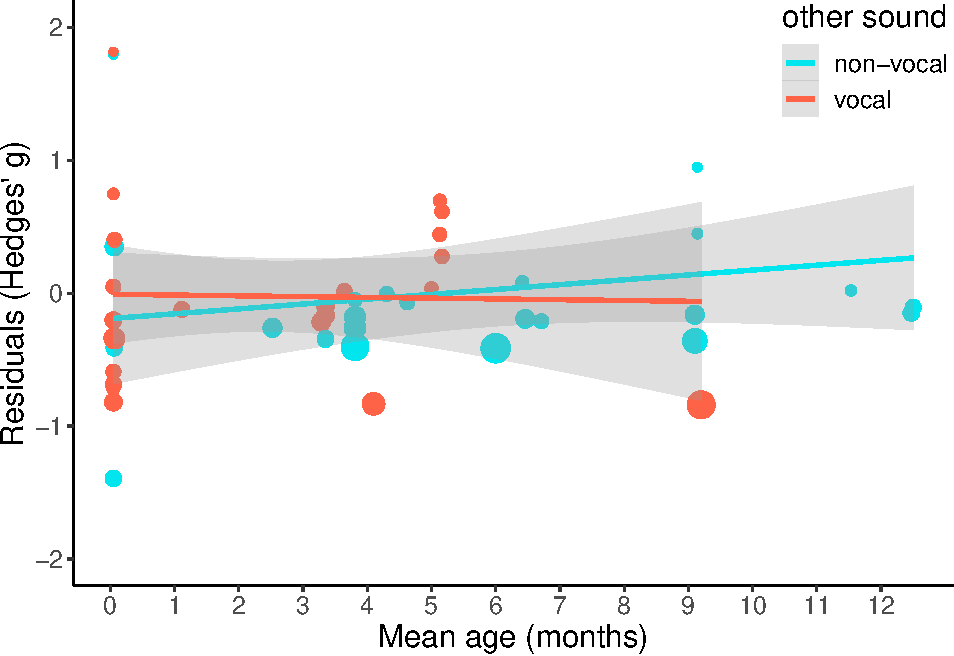
\includegraphics{MA_speech_pref_files/figure-latex/residuals-1.pdf}
\#\#\# Publication bias

We assessed the presence of a potential publication bias in the body of
literature by symmetrizing the funnel plot with the \enquote{trim and
fill} method (Duval, 2005). To do so, we needed to use the simplest
regression, without any moderators. We tested the asymmetry of the
funnel plot by regressing effect size as a function of effect size
standard error and running a Kendall's tau rank test.

\section{Results}\label{results}

\subsection{Database description}\label{database-description}

We found a total of 29 papers reporting 98 (not mutually independent)
effect sizes, see Table 1. All of them have been submitted to or
published in peer-reviewed journals. Studies tended to have small sample
sizes, with a median N of 20 children (Range = 55, M = 21.39, Total:
963). Infants ranged from 0 to 12 months (1.21 to 380.50 days).
Individual samples comprised 42 \% of female participants on average.
Infants were native of 7 different languages across the whole database
(English, French, Japanese, Italian, Russian, Yiddish, Hebrew). Studies
were performed in 13 different laboratories from 6 different countries
(United States, Canada, Israel, France, Japan, Italy). 4 experimental
methods were used: 11 studies used Passive Listening (PL) with
neuro-imaging, with 8 studies using Near-Infrared Spectroscopy (NIRS),
and 3 studies using fMRI; 12 studies used Central Fixation (CF); 3 used
High-Amplitude Sucking (HAS); and 1 used Head-turn Preference Procedure
(HPP).

\subsection{Summary effect size}\label{summary-effect-size}

We found a mean weighted effect size g =0.40 (SE = 0.06 CI = {[}0.27 ,
0.53{]}).

\begin{figure}
\centering
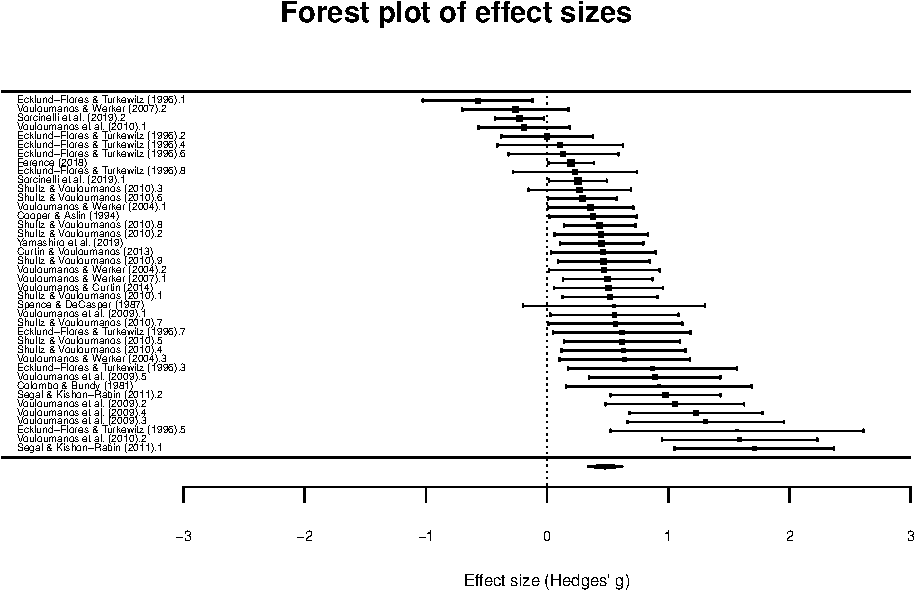
\includegraphics{MA_speech_pref_files/figure-latex/forest plot-1.pdf}
\caption{}
\end{figure}

\subsection{Publication bias}\label{publication-bias}

Evidence of bias at level of papers Evidence of bias at level of
literature

\begin{figure}

{\centering 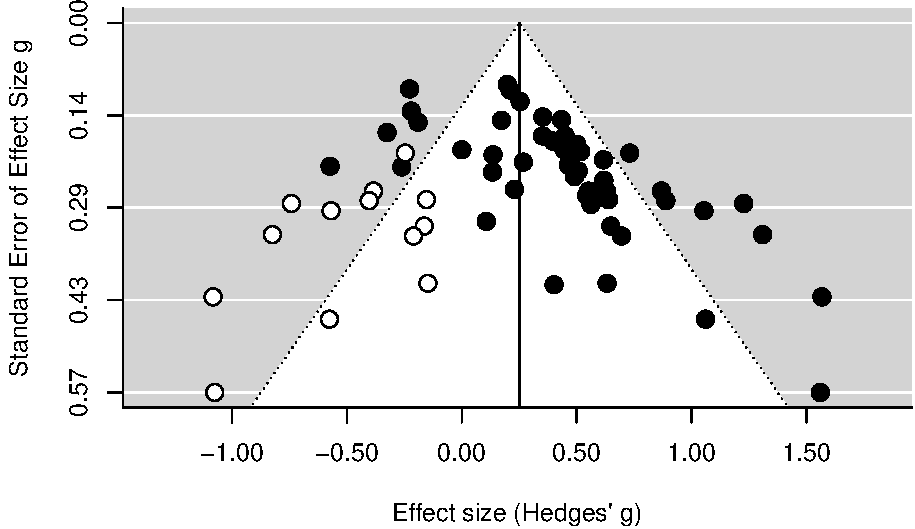
\includegraphics{MA_speech_pref_files/figure-latex/publication bias-1} 

}

\caption{ }(\#fig:publication bias)
\end{figure}

\begin{verbatim}
## pdf 
##   2
\end{verbatim}

\begin{verbatim}
## 
## Rank Correlation Test for Funnel Plot Asymmetry
## 
## Kendall's tau = 0.3550, p < .0001
\end{verbatim}

\subsection{Main effects}\label{main-effects}

\begin{verbatim}
##     HAS      CF     HPP      PL 
## "black"  "blue"   "red" "green"
\end{verbatim}

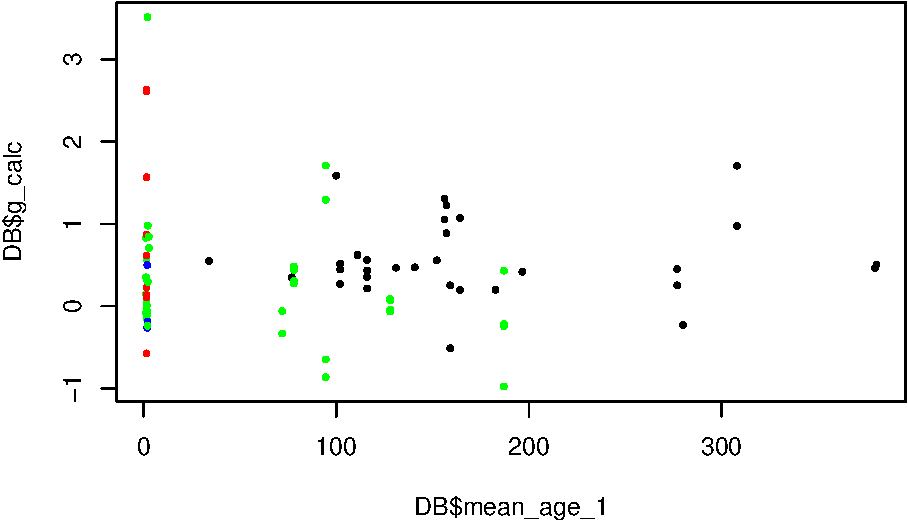
\includegraphics{MA_speech_pref_files/figure-latex/plots-1.pdf}
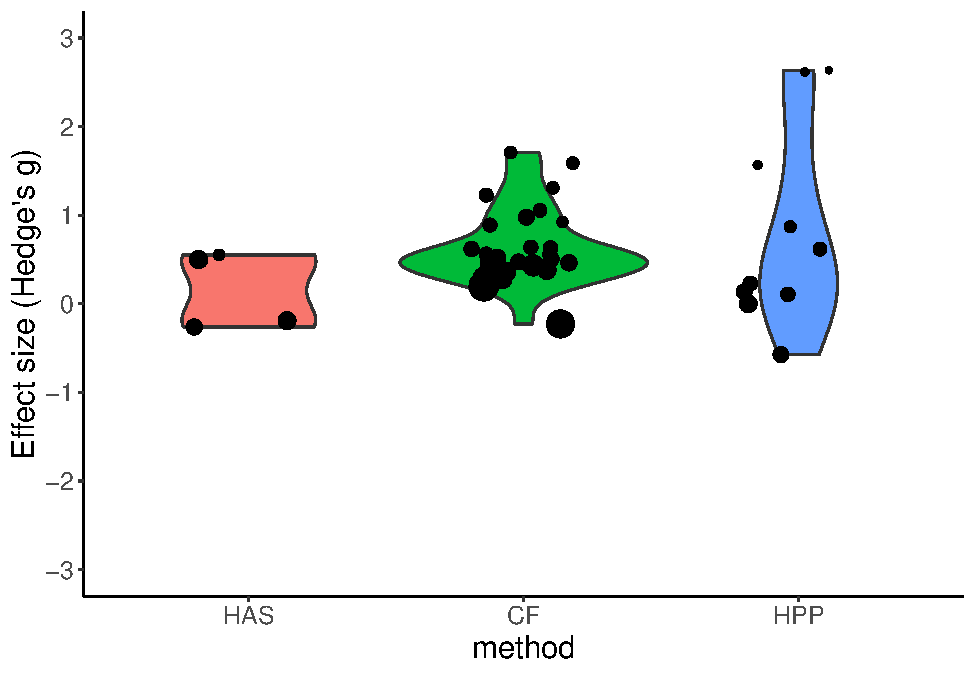
\includegraphics{MA_speech_pref_files/figure-latex/plots-2.pdf}
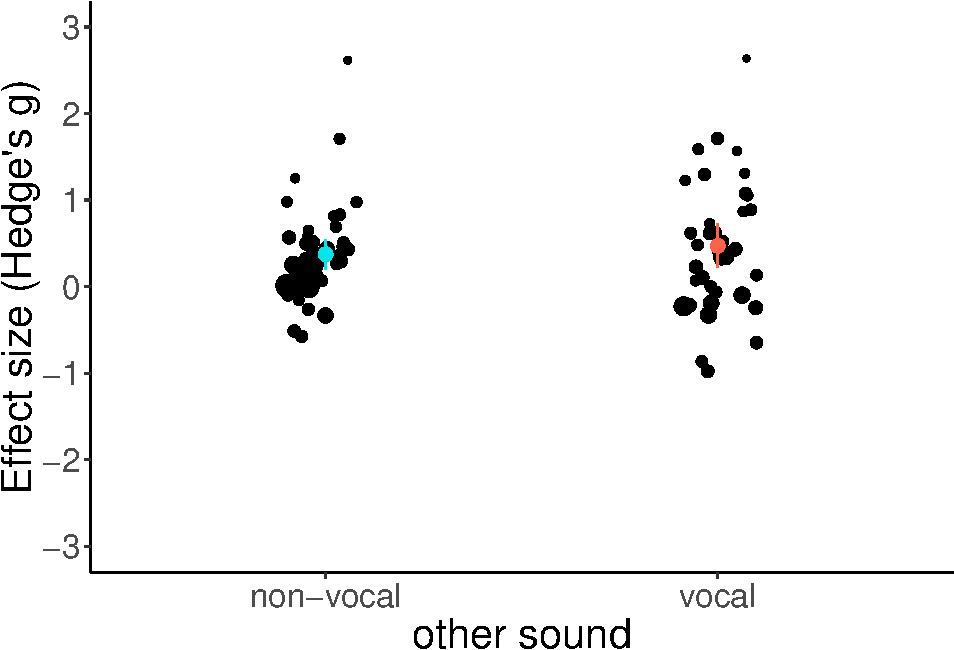
\includegraphics{MA_speech_pref_files/figure-latex/plots-3.pdf}
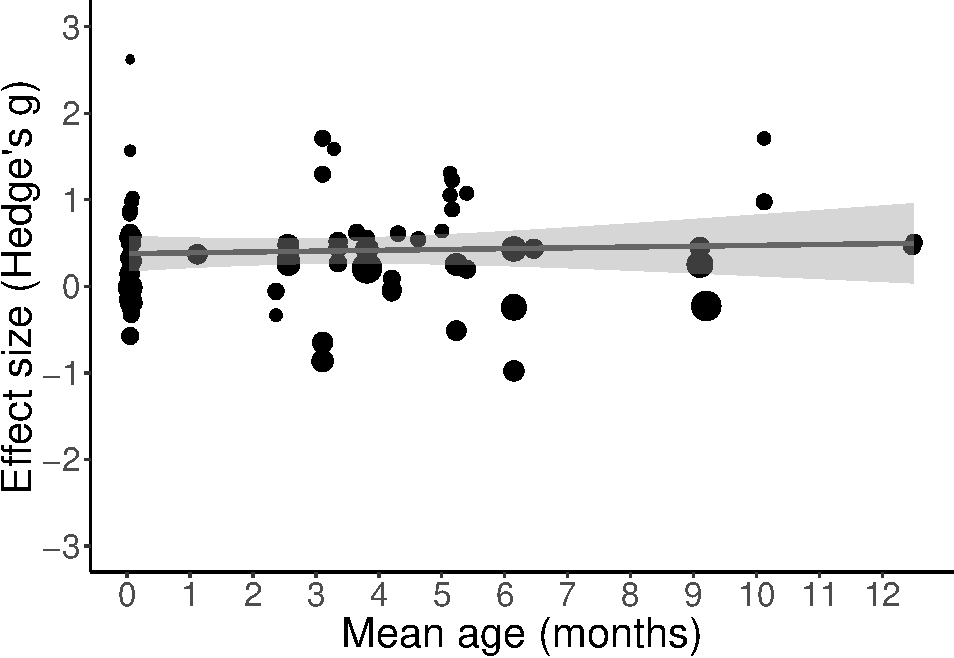
\includegraphics{MA_speech_pref_files/figure-latex/plots-4.pdf}
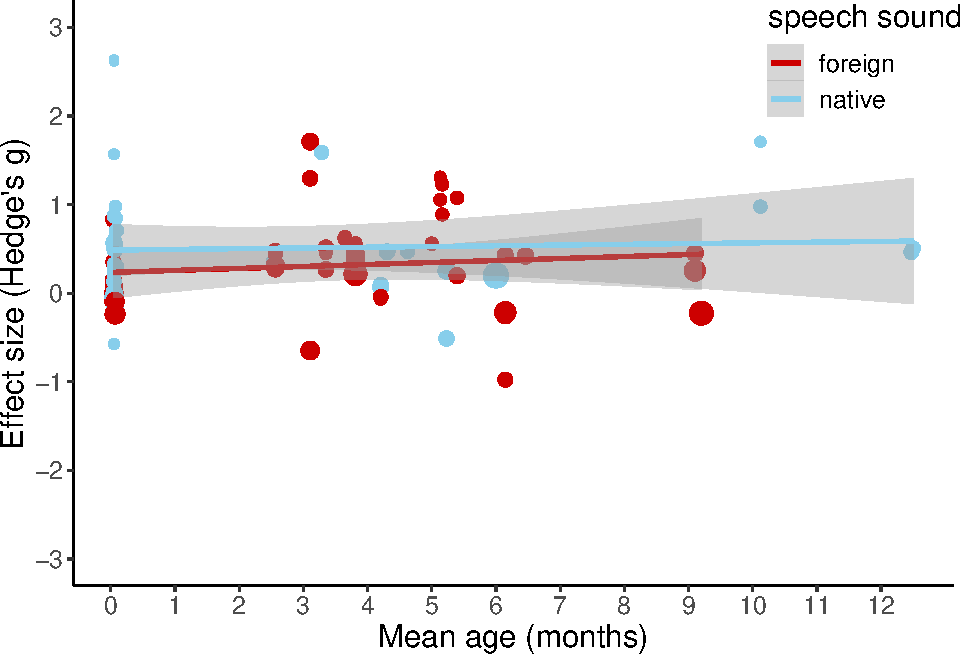
\includegraphics{MA_speech_pref_files/figure-latex/plots-5.pdf}

Heterogeneity Moderators age, type \& interaction

\section{Discussion}\label{discussion}

Our meta-analysis synthesizes the available literature on infants'
preference for speech sound. Our results confirm those of individual
studies, showing that infants reliably prefer speech over other types of
sounds from birth. When all studies were considered together, we found a
sizable intercept at birth. For comparison, the main effect for native
vowel discrimination is estimated at XX (Tsuji \& Cristia, 2013); that
for preference for familiarized words in passages at XX (Bergmann \&
Cristia, ).

A key goal was to interrogate this effect further to assess whether
three potential explanations for it hold up, both at birth and with
potential interactions with age: A preference for natural over
artificial, vocal over non-vocal, and familiar over unfamiliar sounds.
We discuss each in turn.

We reviewed evidence that the auditory system encodes better natural
than artificial sounds (REF), and that naturalness makes a difference
for a higher-level linguistic task, namely word segmentation (Black \&
Bergmann, 2016). In view of such results, we expected infants' speech
preference to be larger when the competitor was an artificial sound than
when it was a natural one. In fact, we found that naturalness alone did
not significantly moderate infants' preference for speech sounds.
Therefore, we can confidently state that a low-level difference in
processing of natural versus artificial sounds is unlikely to explain
away speech preference. speech triggers different cognitive mechanisms
than other sounds. Not incompatible as in this meta-analysis natural
speech stimuli when contrasted to only synthetic speech. We don't know
if infants would have been able to find \enquote{words} with natural
sounds other than syllables (i.e.~frequent sequences of several natural
sounds).

Some previous work had found a preference for speech over other natural
sounds, which may have been indicative of a preference for vocal sounds.
If so, one would have expected greater speech preferences when the
competitor was non-vocal than when it was a vocal sound. Our
meta-analytic regression, however, revealed no significant difference
between these two contrasts.

Do infants show a greater preference for speech when the speech stimuli
are in their native language, than when they are in a foreign language?
For this factor as well, we could not disprove the null hypothesis of no
difference, with widely overlapping distributions of effect sizes for
studies using native as opposed to foreign speech stimuli (controlling
for the competitor via the other factors discussed above).

We hypothesized age to play a major role, not only because it was
correlated with experiences that are crucial for the formation of
categories underlying some of the factors above (e.g., vocalness,
nativeness), but also because it may correlate with a reshaping of the
category definition for speech itself. Indeed, studies comparing
processing of human speech against human non-speech as well as animal
vocalizations more generally (REF, REF) often discuss these age-related
differences in categorization of these sounds. Surprisingly, age did not
significantly moderate the overall preference for speech, and it did not
interact with the other three factors.

There are at least two potential interpretations of the overall pattern
of results. One of them is that, from birth and regardless of changes
co-occurring with age, infants show a preference for speech, which
cannot be reduced to three simpler explanations: naturalness, vocalness,
or familiarity (represented here by the native/foreign contrast). There
exists one simple explanation that we could not test here because there
were not enough studies with appropriate conditions, and that is the
possibility that infants prefer speech because of its complex acoustic
structure and fast transitions. To explore this explanation, it would be
ideal to carry out acoustic analyses of the actual stimuli used in the
studies. Thus, we recommend interested researchers to gather more data
in which the competitor is acoustically simple versus complex; and to
deposit the actual stimuli in a public archive such as the Open Science
Framework (REF). It would also be important to carry out more tests on
infants older than 9 months. Language production gains in complexity at
about this age REF, and it is possible that this would affect infants'
speech preference. We particularly recommend using as competitor natural
vocal stimuli, and as target foreign speech, which would help fill in an
important gap in our dataset.

\begin{verbatim}
More data in general would be helpful also in view of the second potential interpretation of our results: One may wonder whether we fail to find many differences because of a lack of statistical power, particularly in view of between-study variability. We think it unlikely that all null results reported in this paper are due to this for two reasons. First, we did have enough power to detect one main effect, namely experimental method. It has been repeatedly observed in developmental meta-analyses that effect sizes are greatly affected by this variable (see Bergmann et al., 2018, for a synthesis across meta-analysis in developmental psychology). We estimated the effect of method here at about XX. Thus, at the very least, the effects of the factors we studied can be considered to be smaller than this. Second, inspection of results in Figure 3 show that the confidence intervals of all conditions overlap almost exactly. Moreover, Table XX shows that the estimate for all these factors is very close to zero (the maximum being XX). That said, we agree that more data would be welcome.

For interested readers who intend to collect such data, we recommend caution when designing the study, and transparency when reporting it. Another finding of our meta-analysis is that the distribution of effect sizes in the literature is consistent with publication bias, in view of a strong asymmetry of the funnel plot. In fact, the trim-and-fill method suggested 18 points may be missing, which is a considerable number given that we have 82 effect sizes in total (i.e., nearly a quarter more would be missing). Unsurprisingly, the missing studies are in the negative section, i.e., a preference *against* speech, a result that could lead authors to doubt their own data and not submit it to journals, or that would be considered odd by reviewers and editors, who may ask that the data be removed (or who may recommend the paper to be rejected altogether). 

Given the crucial importance of understanding infants' speech preference, we make the following recommendations for further data collection, analysis, and reporting. First, authors should double their sample sizes. The median sample size at present is 20, which is close to the field standard (Bergmann et al., 2018) but much lower than current recommendations (REF). Second, authors should consider proposing their studies as registered reports (REF). This is a new publication scheme (available for journals X Y Z, see a full list on XXX), where manuscripts are submitted before data are collected. Reviewers and editors make publication decisions based solely on the introduction and methods. Once the paper is accepted, the author collects the data, analyses it according to a pipeline described in the accepted methods, and writes up the rest of the manuscript. The paper is then reviewed once more for readability, but it cannot be rejected if the results are surprising or uncomfortable for the field. Third, for authors who would rather not follow this publication route, we still strongly recommend the use of pre-specified analysis plans. These have the virtue of, when used correctly, allowing both authors and readers to separate confirmation from exploration, reducing the likelihood of inadvertently engaging in questionable research practices (REF), known to increase false positives. Finally, we strongly recommend reviewers and editors to evaluate submitted manuscripts on the basis of the quality of the methods, and not of the results. If a study fails to report a speech preference, or actually reports a preference for the competitor, this may actually reflect the reality of this phenomenon.
\end{verbatim}

Infants' preference for speech is a fascinating phenomenon. Beyond the
human species, the capacity to recognize signals from conspecifics might
be crucial for survival and it may be present in other social species
(e.g.~mice, or great apes). To our knowledge, such studies have not been
carried out, but we hope they are in the future. More specific to our
species, preferential processing of speech may support higher level
cognitive tasks, such as categorization (Waxman, 1997; 2007; 2010,
Ferry). And the preference itself may be a meaningful index of
processing that can be used to identify children at risk REF. For all of
these reasons, it is important to take stock of what we know today. Our
meta-analysis compiled public results on this key phenomenon,
establishing that there is a small to medium effect size associated with
it. This preference was not modulated by age, nor three characteristics
of the stimuli employed (whether the speech was native or foreign;
whether the competitor was natural or artificial, vocal or non-vocal).
The analyses also suggested publication bias, for which recommendations
were made for researchers, reviewers, and editors.

\newpage

\begingroup
\setlength{\parindent}{-0.5in} \setlength{\leftskip}{0.5in}

\hypertarget{refs}{}

\endgroup


\end{document}
